\documentclass[../monografia.tex]{subfiles}

\begin{document}

\section{Revisão da Literatura} 

\section{Tecnologias Relevantes} 
\subsection{Protocolos de Rede} 

Com o crescimento do conceito de Internet das Coisas, novas tecnologias para conexão rápida, segura e fácil de dispositivos são criadas e utilizadas por desenvolvedores em inúmeras aplicações. Segundo a pesquisa \textit{Embedded Markets Study} realizada pela empresa Aspencore\cite{embedded-market-study} e apresentada pelos meios EETimes\cite{eetimes} e Embedded\cite{embedded} em 2019, as interfaces sem fio mais utilizadas por desenvolvedores em  projetos de sistemas embarcados são Wi-Fi, \textit{Bluetooth Low Energy (BLE)} e \textit{Bluetooth Classic}. Essa pesquisa também aponta os protocolos de comunicação sem fio mais utilizados, dentre eles \textit{BLE mesh}, Zigbee, 6LoWPAN e Thread. 

Wi-Fi é uma família de tecnologias designadas para comunicação sem fio baseada no padrão IEEE 802.11\cite{802.11}, amplamente utilizada em redes de área local (em inglês \textit{local area network}, LAN) para prover acesso à internet como uma alternativa à tecnologia cabeada Ethernet. Essa tecnologia opera nas faixas de 2,4GHz e 5GHz, sendo que a primeira permite uma taxa de transmissão de até 600 Mbits/s e a segunda até 1 Gbit/s em casos mais extremos\cite{Wi-Fi-datarate}. A topologia comum de uma rede Wi-Fi é dada por um  dispositivo que atua como ponto de acesso que disponibiliza o sinal sem fio para que dispositivos ao seu redor possam se conectar à rede, em uma topologia de rede em estrela. Deste modo, os dispositvos têm que estar a uma distância de poucos metros do ponto de acesso para que a comunicação não seja afetada, sendo essa distância cerca de 76m a 122m em ambientes internos\cite{wifi-range}, dependendo da antena utilizada.

Outra norma comumente utilizada em redes sem fio é a IEE 802.15.4, que define especificações de camada física para redes de comunicação sem fio que operam com baixa taxa de transmissão de dados (em inglês, \textit{Lower Rate Wireless Personal Area Network,}, ou LR-WPAN), que também utiliza a banda de frequência de 2,4GHz\cite{802.15.4}. Os nós participantes da rede podem ser do tipo "função completa" (em inglês, \textit{full-function device} (FFD)), agindo como coordenador da rede, podendo retransmitir mensagens para outros nós, ou do tipo "função reduzida" (em inglês, \textit{reduced-function device} (RFD)), destinados a serem dispositivos simples e com poucos requisitos de comunicação, podendo apenas se comunicar com FFDs. As especificações Zigbee e 6LoWPAN são baseadas nessa norma.

Por último, dentre as tecnlogias citadas anteriormente, o Bluetooth surgiu com objetivo inicial de substituir a conexão por fios entre dispositivos móveis comuns como celulares e fones de ouvido, porém já evoluiu muito e pode ser encontrada em diversas aplicações. Em 2009, a \textit{Bluetooth Special Interest Group} (Bluetooth SIG, organização que gerencia o desenvolvimento do padrão Bluetooth) definiu uma nova versão de baixo consumo energético, chamada de \textit{Bluetooth Low Energy} (BLE), visando aplicações em que não é necessária comunicação contínua como, por exemplo, sensores que coletam dados em intervalos de tempo espaçados. O BLE vem se tornando uma das principais tecnologias para aplicações IoT, principalmente por estar presente na maioria dos dispositivos mais comuns utilizados no dia-a-dia das pessoas, como computadores, \textit{smartphones} e \textit{tablets}, o que facilita a comunicação do usuário com outros dispositivos específicos. As aplicações BLE operam a 2,4GHz com taxas de transmissão entre 0,27 e 1,37 Mbps\cite{ble-datarate}.

Os protocolos citados possuem, em geral, topologias de rede baseadas em estrela, com vários dispositivos periféricos conectados a um central, ou em árvore, que pode ser vista como várias redes em estrela interconectadas. No segundo caso, apenas os dispositivos centrais de cada rede em estrela poderia se comunicar com as outras, atuando como um dispositivo de borda. Desse modo, a conexão entre dispositivos periféricos e central da rede se dá de forma ponto-a-ponto, o que gera uma dependência forte do central e, caso ele apresente algum problema, pode afetar o funcionamento da rede inteira.


\begin{figure}[h!]
\centering
\begin{minipage}{.5\textwidth}
	\centering	
	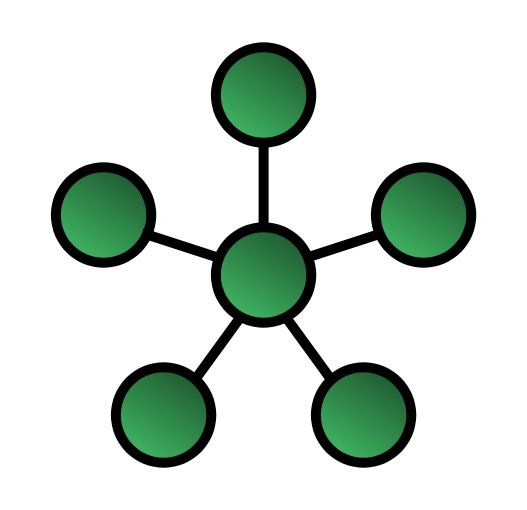
\includegraphics[width=.4\linewidth]{star-network}
	\caption{Topologia de rede em estrela}
	\label{fig:Rede em estrela}
\end{minipage}%
\begin{minipage}{.5\textwidth}
	\centering
	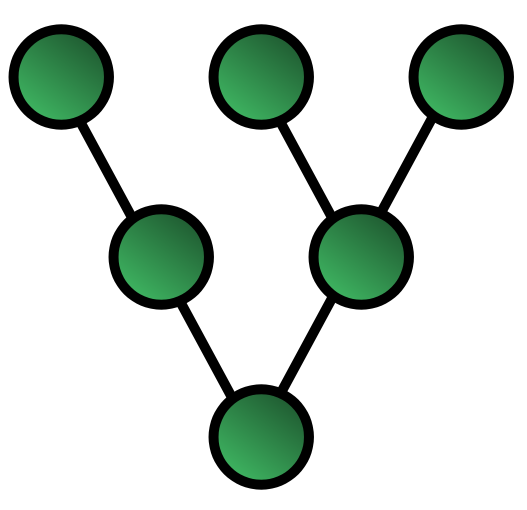
\includegraphics[width=.4\linewidth]{tree-network}
	\caption{Topologia de rede em árvore}
	\label{fig:Rede em árvore}
\end{minipage}

\end{figure}


O crescimento e evolução das aplicações IoT requer topologias mais novas e complexas, com a capacidade de se ajustarem dinamicamente caso ocorra alguma mudança na rede. Com isso em mente, soluções de redes em malha começam a surgir nos protocolos anteriormente citados. Nessa topologia, os nós ficam interligados de forma não-hierárquica, permitindo a comunicação \textit{many-to-many} entre os dispositivos da rede, possibilitando que dados de um ponto qualquer seja enviado a outro ponto qualquer da rede. 


\begin{figure}[h!]
\centering
	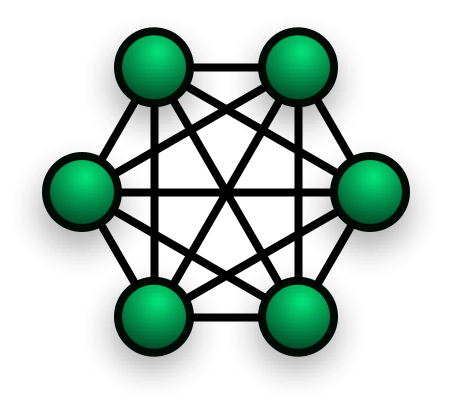
\includegraphics[scale=.2]{mesh-network}
	\caption{Topologia de rede em malha}
	\label{fig:Rede em malha}
\end{figure}

Dada essa necessidade, as epecificações dos protocos de comunicação começaram a adicionar soluções de rede em malha, como BLE Mesh, 802.11s (Wi-Fi mesh) e Thread, que é construída em cima da especificação 6LoWPAN. O protocolo Zigbee já possui suporte a redes em malha desde sua primeira concepção.

O artigo \textit{Wireless Mesh Networking: An IoT-Oriented Perspective Survey on Relevant Technologies}, publicado pela \textit{Future Internet}\cite{mesh-net-comparison} faz uma análise comparativa entre diferentes tipos de protocolos de comunicação atuando na topologia de rede em malha: família IEEE 802.15.4 (Zigbee e Thread), IEEE 802.11 (em especial a IEEE 802.11s que define redes em malha), LoRa Mesh e IEEE 802.15.1 (BLE Mesh).

\begin{figure}[h!]
\centering
	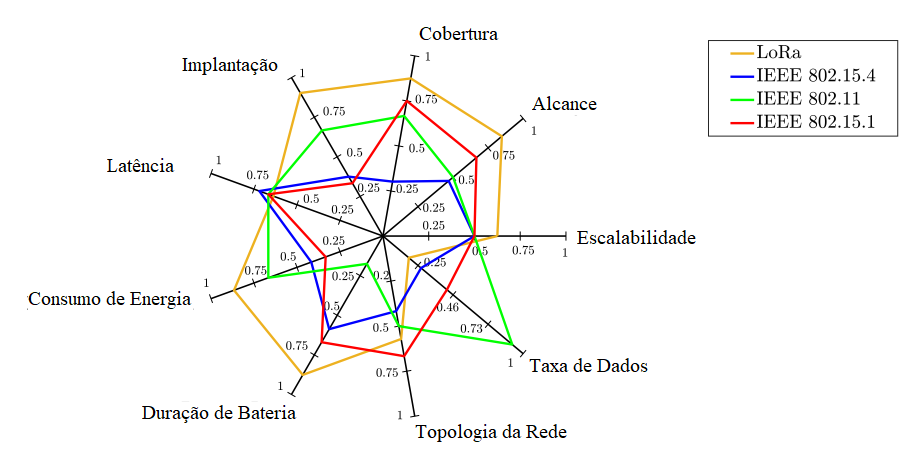
\includegraphics[width=\textwidth]{mesh-net-comparison}
	\caption{
		Comparação de performance entre 4 tecnologias de rede sem fio, em topologia de malha, de acordo com 9 parâmetros. Retirado de \cite{mesh-net-comparison} (traduzido).
	}
	\label{fig:Comparação redes mesh}
\end{figure}

O gráfico mostrado na figura \ref{fig:Comparação redes mesh}  pode ser utilizado para resumir de maneira completa a pesquisa realizada em \cite{mesh-net-comparison}. O protocolo LoRa foge do escopo deste projeto, pois é destinado para comunicações entre distâncias quilométricas e possui taxa de transmissão de dados muito baixa, por isso será desconsiderado como alternativa para a aplicação deste projeto. É possível observar os seguintes pontos:

\begin{itemize}
	\item A tecnologia Wi-Fi é claramente a que possui maior taxa de transmissão de dados, com área de cobertura e alcance razoáveis, mas com a desvantagem de possuir um consumo de energia elevado.
	\item Redes BLE Mesh são as mais eficientes em termos de consumo de energia, mostrado também no artigo \cite{zigbee-ble-power}, possuem grande área de cobertura, já que uma rede pode possuir até 32 mil nós\cite{BLE-mesh}, e possuem uma taxa de trasmissão de dados alta, comparada com as soluções baseadas na IEEE 802.15.4.
	\item Todas as soluções apresentadas possuem alta escalabilidade e níveis de latência comparáveis.
\end{itemize}


\section{Soluções no Mercado} 
% Falar de ser Open Source

A tabela a seguir mostra algumas das principais soluções encontradas no mercado para monitoramento de ambientes fechados: 

\begin{center}
\begin{tabular}{ | m{2.5cm} | m{2.4cm}| m{2.2cm} |m{2cm} |m{2cm} |m{2.8cm} | } 
\hline
\textbf{Projeto} & \textbf{Térmico} & \textbf{Luminoso} & \textbf{Acústico} & \textbf{Ar} & \textbf{Conectividade} \\ 
\hline
Multi comfort \cite{multicomfort} & Sim* & Sim* & Sim* & Sim* & Sim* \\ \hline
MC350\cite{mc350} & Sim* & Sim* & Sim* & & Bluetooth, App \\
\hline
Metriful Sense\cite{metriful} & Temperatura, Umidade, Pressão & Intensidade & Volume, Freq. & VOC &  \\ \hline
CoMoS\cite{CoMoS} & Temperatura, Umidade, Veloc Ar & Intensidade & & & Wifi, SW Web \\ \hline
HC tech\cite{HCTech} & Temperatura, Umidade & Intensidade & & & Sigfox, SW Web \\ \hline
ECOMLITE \cite{ECOMLITE} & Temperatura, Umidade, Pressão & & Volume & $CO_{2}$, CO, VOC, $NO_{2}$ & Wi-fi, Zigbee, Ethernet, SW Web \\ \hline
Netatmo\cite{netatmo} & Temperatura, Umidade, & & Volume & CO2 & Wi-fi, App \\ \hline
Senlab O\cite{Senlab} & Temperatura, Umidade & Intensidade & & & LoRa \\ \hline
Comfort Click\cite{comfortclick} & Temperatura, Umidade & & Volume & & Wi-fi, App  \\ \hline
\end{tabular}
\end{center}

\begin{flushright}
(*) Solução não detalhada pela construtora
\end{flushright}


% Análise  - Finalizar
Ao observar as soluções existentes no mercado, é possível ver que a maioria atende a apenas alguns dos indicadores. 

Multi Comfort \cite{multicomfort}, a solução mais completa encontrada, trata-se de uma sistema desenvolvido pela construtora Saint-Gobain de forma integrada à construção do edifício. Como apresentado pelo prof. Vanderley (PCC), o monitoramento e automação na construção civil vem crescendo nos últimos anos, de forma que soluções desse tipo tendem a tornar-se mais comuns. 
Apesar de atender aos 4 indicadores de qualidade e conforto, essa solução não apresenta detalhes sobre as medições que são feitas, quais os elementos medidos ou a precisão dessas medições, assim como sobre a sua conectividade. Também apresenta grande dificuldade para integração em um ambiente já construído. Nesse contexto, é introduzido o equipamento MC350\cite{mc350} - da mesma empresa -, mas que não atende mais a todos os indicadores. 

Em seguida, temos o Metriful Sense \cite{metriful}, que também atende a todos os indicadores de conforto, que é um produto novo em \textit{crowdfunding}. Diferentemente das demais, esse não é um dispositivo completo, mas uma plataforma de sensores projetada para o monitoramento de ambientes, que necessita de uma interface com outro processador e possivelmente com um módulo \textit{wireless} para que haja conexão com uma plataforma de análise. 

Os demais produtos atendem em média apenas dois dos indicadores de conforto, sendo apenas o conforto térmico presente em todos. O conforto luminoso, quando presente, é atendido de forma superficial, sendo medida apenas a intensidade da luz e não a temperatura, que é um elemento importante na sensação de conforto \cite{VisualComfort}. Já no monitoramento da qualidade do ar, apenas uma das soluções \cite{ECOMLITE} (cuja especificação está disponível) mede ao menos os dois principais elementos indicadores \cite{AirQuality}. 

Vemos, assim, que nenhum dos produtos existentes no mercado atende a todos os requisitos levantados para a nossa aplicação. A proposta aqui é o desenvolvimento de um dispositivo que monitore a qualidade e o conforto do ambiente atendendo a todos os indicadores apresentados de forma completa, e com uma medição mais aprofundada em conforto luminoso e qualidade do ar que os projetos comparados. 

Além disso, nenhuma das soluções encontradas envolve diretamente a opinião das pessoas frequentando o ambiente na análise dos seus dados, apenas no controle do ambiente quando esse não atende os requisitos de qualidade ou de conforto. 

Vale destacar, por fim, que na maioria dos casos essas soluções são fechadas, com protocolos que dificultam a integração dos dispositivos com outros que possam complementá-los em seu funcionamento, ou de forma que seja possível uma centralização da análise dos dados coletados. Desenvolvendo um projeto \textit{open-source} e com protocolos padrão de comunicação sem fio, isso deixa de ser um problema. 

\section{Árvore de Objetivos} 
% arvore de objetivos
A árvore de objetivos é uma representação gráfica dos meios necessários, chamados objetivos específicos, para alcançar o objetivo geral do projeto. Para atingir o objetivo geral do projeto, que é a realização de uma rede de dispositivos para monitorar ambientes, foram enunciados três objetivos específicos, mostrados na figura \ref{fig:objective-tree}, com a porcentagem de dedicação ao lado de cada um.

\begin{figure}[h!]
%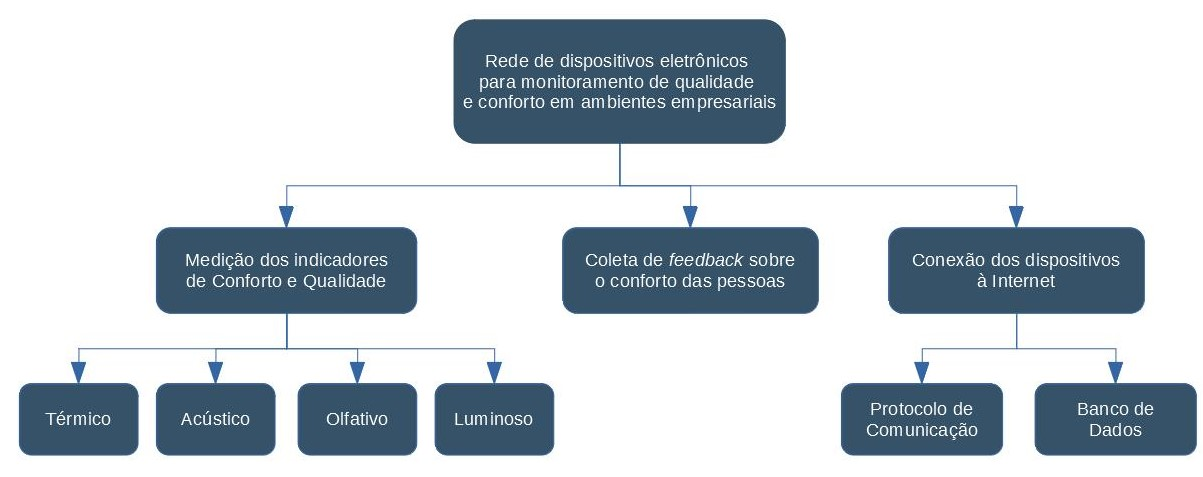
\includegraphics[scale=0.65]{objective_tree}
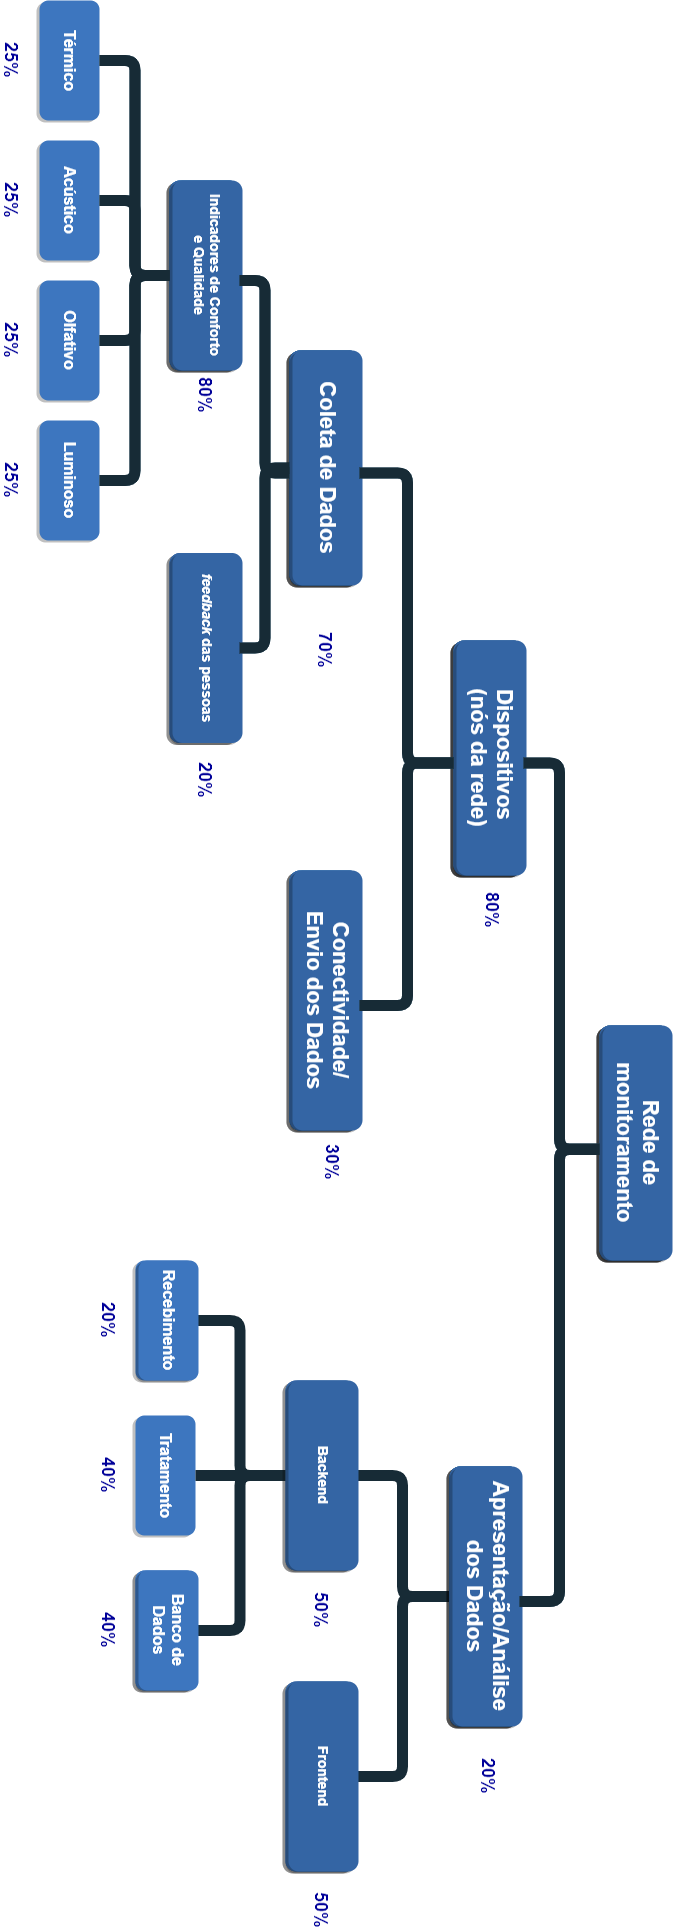
\includegraphics[width=\textwidth]{objective-tree-2}
\caption{Árvore de objetivos do projeto}
\label{fig:objective-tree}
\end{figure}


\end{document}